% =====================================================================
\chapter{Introduction}
\label{ch:intro}
% =====================================================================

\section{Motivation}

A large language model, hereafter abbreviated LLM, is a neural network trained to
predict the next token in a sequence of text. Once trained on enough data, such a model
can answer questions, summarise documents, and hold a conversation. The same property
that makes these systems useful also makes them dangerous in a specific way: they are
optimised to produce text that \emph{looks} right, not text that \emph{is} right. As a
result, an LLM will sometimes state a wrong fact with the same fluency and confidence
that it uses for a correct one. This behaviour is widely called \emph{hallucination},
and a now-standard survey of the topic describes it as the generation of content that
is fluent and plausible yet unfaithful to the source or to the world~\cite{ji2023survey}.

Hallucination is not a rare glitch. It is a structural consequence of how these models
are built, and it appears across every task to which LLMs are applied. When a model
invents a citation, misstates a medical dosage, or confidently answers a question whose
premise is false, the cost is borne by whoever trusted the answer. As LLMs move from
demonstrations into tools that professionals rely on, the ability to attach a warning
to an unreliable answer becomes as important as the answer itself. The problem this
dissertation addresses is therefore not how to stop a model from hallucinating, but how
to \emph{detect}, cheaply and in real time, when it probably has.

Several families of detectors exist, and we review them in detail in
Chapter~\ref{ch:related}. One popular family samples the model many times and checks
whether the answers agree, on the intuition that fabricated content is unstable while
real knowledge is consistent; the best-known method of this kind is
SelfCheckGPT~\cite{manakul2023selfcheckgpt}. This approach works without any access to
the model's internals, but it is expensive: it requires many full generations for every
single answer it checks. A second family takes the opposite view. It assumes we can open
the model up and read the hidden activations it produces while generating, and it learns
a small classifier that maps those activations to a hallucination probability. The
appeal is cost. Because the activations are already computed during normal generation,
reading them adds almost nothing to the running time. Figure~\ref{fig:latency}
illustrates the gap that motivates this entire line of work: a sampling-based check can
cost hundreds of times more per response than an internal-state probe.

\begin{figure}[t]
\centering
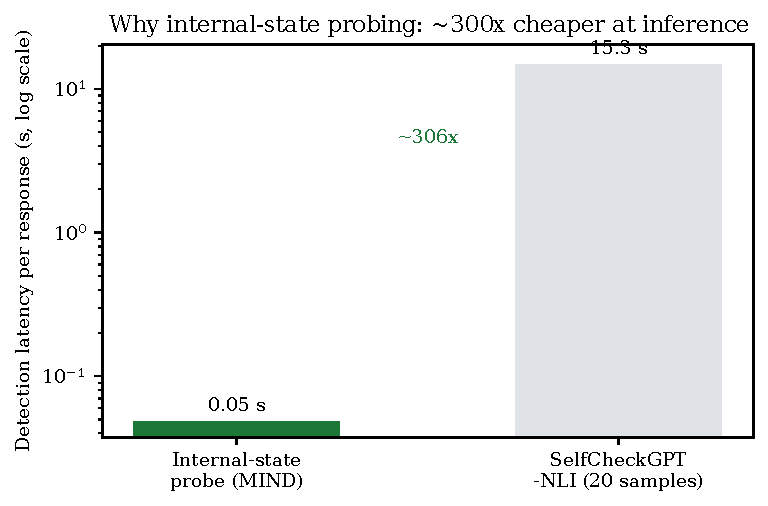
\includegraphics[width=0.62\textwidth]{images/ch01_intro/ch01_1_latency.pdf}
\caption{The practical case for internal-state probing. A consistency check that draws
roughly twenty extra samples per response costs orders of magnitude more time than a
classifier that reads activations the model has already produced. Latencies are
indicative figures from the internal-state detection literature, plotted on a
logarithmic scale.}
\label{fig:latency}
\end{figure}

The internal-state family began with the observation that a model's hidden layers seem
to ``know'' when the model is producing a falsehood, even when its surface output gives
no hint~\cite{azaria2023saplma}. Building on this, the MIND framework showed that one
can generate the training labels automatically, rather than by hand, and still train an
effective and fast detector~\cite{su2024mind}; here MIND refers to the model
internal-state-based detection method of Su et al., which we adopt as our starting
point. Later work pushed the idea further, either by removing the need for any labels at
all~\cite{du2024haloscope} or by fusing signals from every layer of the
network~\cite{dasgupta2025hallushift}. These methods are promising, but they have been
reported under inconsistent conditions, and crucially most of them were demonstrated on
large models running on research-grade hardware. Whether the same signals survive on
the smaller open models that a student or a small team can actually run, and how the
many proposed features compare on equal footing, is the gap this dissertation sets out
to fill.

\section{Problem Statement}

The central question of this work can be stated plainly:

\begin{quote}
\emph{Given an open-weights language model running on free, memory-limited hardware, how
reliably can we detect hallucinations by reading internal representations from a single
forward pass, and which internal-state signals are worth their cost?}
\end{quote}

This question has three parts that are easy to conflate and that we deliberately keep
separate throughout the dissertation. The first part is the \emph{detection signal}:
which quantities, computed from the hidden states and the output distribution, carry
information about whether the current generation is faithful. The second part is the
\emph{evaluation regime}: a detector trained on one kind of text (here, automatically
labelled encyclopedia continuations) may work well on similar text but transfer poorly
to question answering, summarisation, or dialogue. Reporting a single headline number
hides this distinction, so we always separate held-out in-distribution performance from
cross-task transfer. The third part is the \emph{compute budget}: a method that needs
multiple samples, a singular-value decomposition, or a large auxiliary model may be
accurate but impractical on the hardware we target. A useful detector has to be honest
on all three axes at once.

A complication specific to this work is that a closely related study exists at the same
institute, conducted independently in a different research group, which targets the same
benchmark suite. To keep the present contribution clearly its own, the design of our
detector deliberately differs from that prior study at the level of features and
classifier; this separation is explained where the relevant method is introduced in
Chapter~\ref{ch:related} and respected throughout.

\section{Research Objectives}

The objectives of the dissertation are the following.

\begin{enumerate}[leftmargin=2.2em,itemsep=0.3em]
\item To re-implement the label-free, internal-state detection pipeline of the MIND
framework~\cite{su2024mind} so that it runs end to end on free cloud GPUs, and to verify
its correctness with a small diagnostic model before scaling up.

\item To design three inexpensive internal-state features --- layer-wise representation
drift, cross-layer variance, and predictive entropy --- that are computed from the same
forward pass as the existing canonical feature, and to define them in clean,
self-contained notation.

\item To assemble a single ablation that compares the canonical feature, the three new
features, a set of nine features drawn from the recent literature, and a further set of
exploratory features, under one fixed classifier and one fixed evaluation protocol.

\item To evaluate this ablation against four established baselines and two simple
reference methods across a multi-task benchmark suite spanning question answering,
summarisation, and dialogue, on several open models of different sizes.

\item To report the outcome honestly: to state which numbers are backed by saved
measurements, to keep in-distribution and transfer results apart, and to avoid any claim
of superiority that the measurements do not support.
\end{enumerate}

\section{Thesis Contributions}

The contributions of this dissertation are modest by design and are stated as such.

\textbf{A free-tier-reproducible comparison.} The primary contribution is a unified,
reproducible comparison of internal-state hallucination features across multiple open
LLMs, built to run within the memory and time limits of free cloud notebooks. Every
configuration shares the same automatically generated training data, the same
classifier, the same train/test split, and the same evaluation rows, so that
differences in measured performance can be attributed to the features rather than to
incidental differences in setup.

\textbf{Three forward-pass features and a clean ablation.} We introduce three
additional internal-state signals on top of the canonical hidden state and place them
in an ablation alongside literature features and exploratory features. The ablation
isolates what each family of features adds, rather than reporting only a single combined
system.

\textbf{An honest, regime-separated account of the results.} We show that, on the model
for which we have a complete set of measurements, the richer feature configurations are
competitive with the strongest baseline but do not surpass it, and that a single
benchmark dominates the averages. We further show that cross-task transfer is markedly
harder than in-distribution detection. We treat these findings, including the ones that
are unflattering to the proposed features, as the result.

It is worth stating clearly what this dissertation does \emph{not} claim. It does not
claim a new state-of-the-art detector, it does not claim to beat any prior method on its
own benchmark, and it does not present results for experiments whose measurement files
are not yet complete. Where an experiment is still running, it is marked as pending.

\section{Thesis Organization}

The remainder of the dissertation is organised as follows.

\textbf{Chapter~\ref{ch:background}} provides the background needed to read the rest of
the work: how transformer language models produce hidden states, what a hallucination is
in precise terms, and how detection is measured.

\textbf{Chapter~\ref{ch:related}} surveys the literature on hallucination detection,
organising it into four families and positioning the present work within the
internal-state family. It is here that the related institute study is cited once, as
adjacent prior work, with an explicit account of how our method differs.

\textbf{Chapter~\ref{ch:method}} presents the methodology: the automatic label
generation, the canonical feature and the three new internal-state features in full
notation, the wider feature families, the classifier, the baselines, and the
free-hardware implementation.

\textbf{Chapter~\ref{ch:results}} reports the experiments. It presents the verified
results, separates in-distribution from transfer performance, discusses the strengths
and weaknesses of the proposed features, and marks the experiments that are still in
progress.

\textbf{Chapter~\ref{ch:conclusion}} summarises what was found, states the limitations
without softening them, and lays out concrete next steps.
